% This is samplepaper.tex, a sample chapter demonstrating the
% LLNCS macro package for Springer Computer Science proceedings;
% Version 2.21 of 2022/01/12
%
\documentclass[runningheads]{llncs}
%
\usepackage[T1]{fontenc}
% T1 fonts will be used to generate the final print and online PDFs,
% so please use T1 fonts in your manuscript whenever possible.
% Other font encondings may result in incorrect characters.
%
\usepackage{graphicx}
\usepackage{mdframed}
\usepackage[normalem]{ulem}
\usepackage{hyperref}
% Used for displaying a sample figure. If possible, figure files should
% be included in EPS format.
%
% If you use the hyperref package, please uncomment the following two lines
% to display URLs in blue roman font according to Springer's eBook style:
%\usepackage{color}
\renewcommand\UrlFont{\color{blue}\rmfamily}
%

\newcommand\todo[1]{\textcolor{red}{TODO: #1}}
\graphicspath {{../res}}
\begin{document}
%
\title{Sophize Mathematics Library}
%
%\titlerunning{Abbreviated paper title}
% If the paper title is too long for the running head, you can set
% an abbreviated paper title here
%
\author{Abhishek Chugh\inst{1}\orcidID{0000-0001-6765-5229}}
%
% First names are abbreviated in the running head.
% If there are more than two authors, 'et al.' is used.
%
\institute{Sophize Foundation, Bengaluru - 560066, India 
\email{abc@sophize.org}
}
%
\maketitle              % typeset the header of the contribution
%
\begin{abstract}
Sophize is a novel mathematics library and discussion platform with a mission to help our
users find and organize mathematical proofs. We present Sophize's novel yet familiar
knowledge organization scheme that is used to represent a wide variety of proofs. With this
scheme at its core, we have engineered a platform to logically aggregate knowledge from
multiple sources. The platform curates knowledge from published research, encyclopaedias
such as PlanetMath and Wikipedia, informal computer programs, and formal systems such as
Metamath; and allows its users to run a federated search over them. To make this happen, two
developments were necessary. First, we came up with the concept of 'proof-generating
machines' and developed an open plugin architecture that allows proofs from computer
programs to be generated as required. Second, we extended the Markdown language to represent
the connections between mathematical objects found across various sources of knowledge. In
addition, we also utilized this new language to create a novel communication system built
specifically to aid mathematicians in solving problems collaboratively.


\keywords{Sophize \and
knowledge organization \and
proof-generating machine \and
belief set \and
metamath \and
markdown \and
argument graph \and
proof graph \and
semantic data}
\end{abstract}


\section{Introduction}

\subsection{The Sophize Platform}


Sophize is a novel mathematics library and discussion platform. The author has developed the
platform over the course of the last few years at \url{https://sophize.org}. Sophize's
primary mission is to help users find existing proofs of mathematical statements, to
discover new proofs, and to utilize this knowledge in their work. We combine knowledge from
multiple resources and have accumulated thousands of definitions, theorems, and proofs from
a wide variety of sources, including some published research, the PlanetMath encyclopedia,
Wikipedia, and the Metamath formal system \cite{metamath}.

\subsection{Motivation}

In the past couple of decades, the Internet has revolutionized our life by giving us access
to seemingly unlimited information. Information from a wide variety of topics ranging from
human medicine to rocket science is now just a few keystrokes away. However, it seems
that we are having even more trouble making sense of the World around us. In fact, dealing with the vast amounts of information thrown at us seems to be one of the most important problems of our generation. While we have access to a wide range of opinions on almost every topic imaginable, it has become increasingly difficult to decide which one to trust. It
seems that we can find "proofs" for anything and everything we would like to believe.

Thus the author's primary motivation for this project is to create a library that not just
lays out all the information about the World but organizes it in a way that helps us make
better sense of it. A library that helps us access justifications from a variety of
viewpoints and allows us to collaboratively and objectively evaluate issues in the
justifications or the viewpoints they arise from. Clearly, this is a challenging goal. 

We begin our journey with a focus on pure Mathematics, where knowledge is objectively less
complex as compared to other fields. In mathematics, only logically sound arguments are
acceptable as justifications. These arguments develop in different foundational theories;
and logical consistency is the primary criterion of correctness. Thus, as a
Mathematics library, Sophize's goal is to help our users access mathematical proofs (arguments) from a variety of belief sets (roughly - foundational theories along with indicators of trust in knowledge sources) and allow our users to collaboratively and objectively evaluate issues in the arguments or the belief sets they developed in.

With our current scheme, we can incorporate nearly all mathematics. A natural extension
would be to model observational data and develop criteria to quantify empirical
correspondence in order to have the ability to incorporate scientific knowledge. But, for
now, we are focused on developing a state-of-the-art library for the Mathematics community.

\subsection{Proofs in Sophize}
\label{sec:sophize_proofs}

\begin{figure}[!ht]
\begin{center}
\fbox{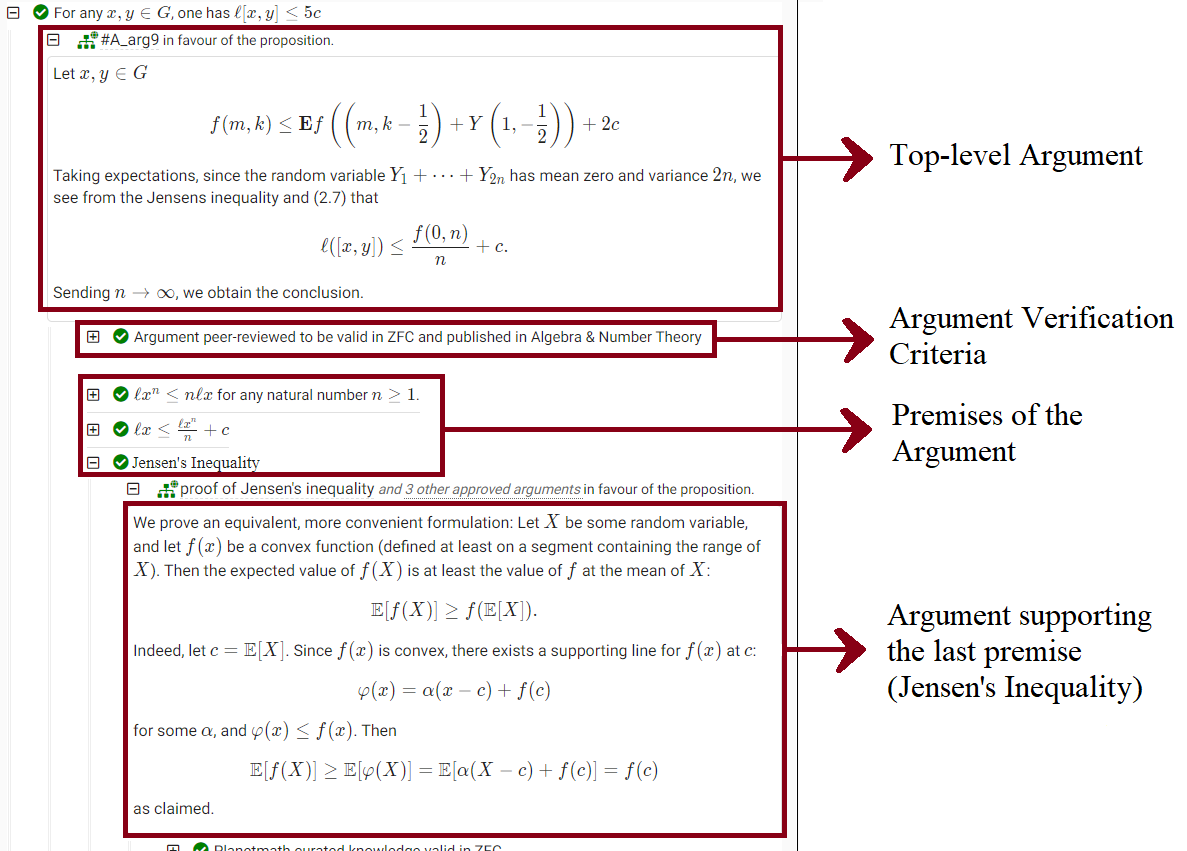
\includegraphics[height=8.25cm]{proof_tree}}
\caption{A proof displayed as a graph (tree) of arguments and propositions on the Sophize platform.}
\label{proof_tree}
\end{center}
\end{figure}


Mathematical proofs are based on a variety of foundations such as ZFC, intuitionistic logic, and type theory. The arguments used in any proof are considered valid or not based on criteria that can vary. Most academic mathematics is peer-reviewed and published, but some mathematical proofs can be found in community curated sources such as Wikipedia. Proofs can also be algorithmically generated, and at the highest level of verification, they are represented and verified using a formal system. 

Sophize combines such an expansive range of proofs into a dense graph of propositions and logical arguments that aggregates knowledge from several documents and other data sources. We use this graph and combine it with the set of foundations and verifications chosen by each user to create proofs tailored to their needs. This introductory video gives an overview of the platform's offerings: \url{https://youtu.be/Wb1JbW9Otek}.

This work can also be seen as a step towards formalizing the network of information that exists in the connections of mathematical objects. The committee on planning a global library of the mathematical sciences recognized that this network is largely unexplored, and formalizing it has tremendous potential to accelerate math research \cite{sciences2014developing}. Hence, we required novel techniques to connect mathematical entities from such a wide range of formal and informal knowledge sources.

\subsection{Contribution}
In this paper, we present the novel concepts and features of Sophize Mathematics Library. First, we expound Sophize's scheme to build a trust-focused logical network of mathematical knowledge. In section \ref{sec:pgm}, we describe Sophize's proof-generating machines which are computer programs that generate proofs that integrate with Sophize's knowledge graphs.

We then present some features of Sophize Markdown, an extension of the Markdown language that helps present Sophize's knowledge graphs to its users. It is convenient enough to be used for casual discussions of mathematical ideas over the web. It is also powerful enough to embed mathematical entities such as definitions, theorems, and proofs from various sources, including formal systems. It thus plays an integral role in the two problems that we have mentioned above.

Section \ref{sec:lib} discusses some other challenges and contributions made towards making Sophize a modern mathematics library. Finally, Section \ref{sec:conclusion} concludes the paper.


\section{Sophize's Knowledge Organization Scheme}
At its core, Sophize's approach is to simply keep track of all arguments in favour or against any proposition. The use of some form of arguments is the common factor amongst all mathematical (and perhaps most scientific) knowledge. We use this fact to unify knowledge from multiple sources in a meaningful way as described below.

We use the set of all known arguments to track knowledge from a variety of foundational theories. For theoretical knowledge, i.e., the knowledge that doesn't involve empirical data, the primary criterion of validity is internal (logical) consistency. Thus, for each foundational theory (`belief set' described below), we also keep track of any contradictions that arise from those foundations.

\subsection{Core Concepts}
\label{sec:core}
Sophize uses the following concepts to logically organize theoretical knowledge. The datamodel for these concepts is published in JSON schema \cite{sophize_datamodel}.

\paragraph{A \textbf{resource} is an abstract concept inherited by all other top-level concepts like terms, propositions, arguments, and belief sets. Each resource has a URI and contains fields such as search tags and citations.}
\paragraph{}
A \textbf{URI} consists of two parts: a namespace-like identifier called its dataset-id, which indicates the data source, and a resource-id that specifies the resource type and its unique name in the data source. The dataset-id may be omitted if it can be inferred from the surrounding context.

For example, the Pythagorean theorem (a \textbf{P}roposition) represented in the Metamath project may have the URI \emph{metamath/\textbf{P}\_pythagorean} and the definition of cone (a \textbf{T}erm) extracted from Wikipedia may have the URI \emph{wiki/\textbf{T}\_cone}. When used inside another resource in the same (`wiki') dataset, cone's definition can be referred to simply as \emph{T\_cone}.

The same URI scheme will be used in this paper to refer to various terms, propositions, arguments, etc.

\paragraph{A \textbf{term} is a clearly defined entity that can be used to make up a valid proposition. It can be a mathematical object, operator, symbol, data structure, algorithm, or even a person. `Meaningless' primitives in formal theories are also categorized as terms.}

\paragraph{A \textbf{proposition} is a grammatically valid statement that can be either true or false. Axioms, theorems, conjectures, hypotheses, lemmas, corollaries, and converses are all classified as propositions.}

\paragraph{An \textbf{argument} is a set of propositions called premises along with a concluding proposition that is claimed to follow from the premises. In addition, most arguments include supporting text that explains how the conclusion follows from the premises.}

\paragraph{A \textbf{belief set} is roughly the set of axiomatic propositions that make up the foundations of a theory. Belief sets will be described in subsection \ref{sec:bset}.}

\paragraph{Loosely defined, a \textbf{proof-generating machine} (PGM) is a computer program that generates proofs for an input proposition on-the-fly. PGMs are described in detail in section \ref{sec:pgm}.}

\subsection{Argument Graph}
An argument can be seen as a simple graph (see Fig.~\ref{argument_graph}) with two types of nodes - (a) a single node representing the argument itself and (b) a set of proposition nodes representing the argument's conclusion and premises. The edges of this graph are directed and go from (a) premise nodes to argument node and (b) argument node to conclusion node. A set of arguments can thus be represented as a single graph that we call an \textbf{argument graph}.

\begin{figure}[!ht]
\begin{center}
\fbox{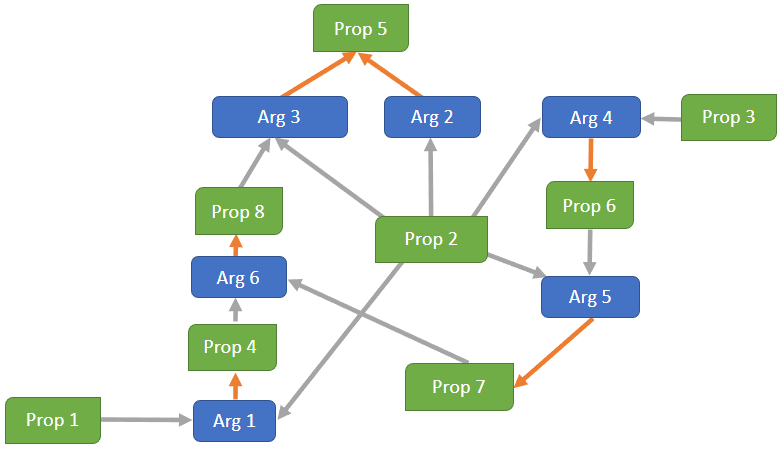
\includegraphics[width=\textwidth]{argument_graph}}
\caption{An argument represented as a graph (left). A set of arguments forming an argument graph (right).}
\label{argument_graph}
\end{center}
\end{figure}


\subsection{Generating Proof Graphs}
A \textbf{proof graph} is a directed acyclic graph and contains complete proofs (including all alternate proofs) for all its propositions. A proof graph can be generated from an argument graph by starting with the axiom nodes and finding all nodes that can be reached from them (See Fig.~\ref{proof_graph1}).


\begin{figure}[!ht] 
\begin{center}
\fbox{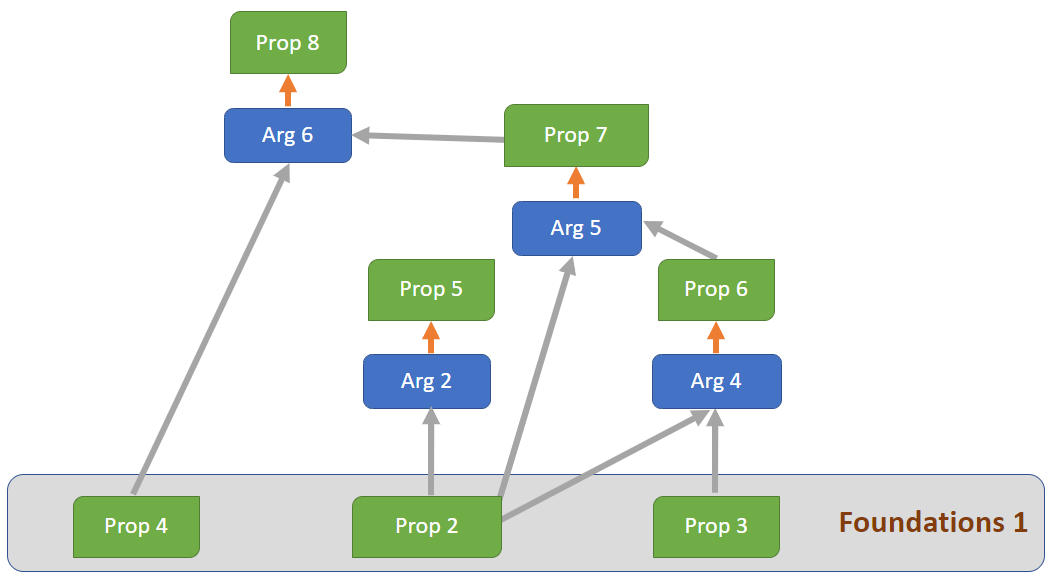
\includegraphics[height=5cm]{proof_graph1}}
\caption{Proof graph from argument graph (Fig.~\ref{argument_graph}) using `Prop 2', `Prop 3', Prop 4' as axioms.}
\label{proof_graph1}
\end{center}
\end{figure}



\begin{figure}[!ht]
\begin{center}
\fbox{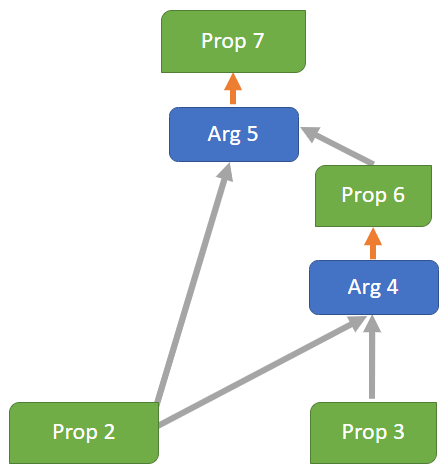
\includegraphics[height=4cm]{proof_prop7}}
\caption{Proof of `Prop 7' from proof graph in Fig.~\ref{proof_graph1} uses `Arg 4' and `Arg 5'.}
\label{proof_prop7}
\end{center}
\end{figure}

Note that an argument graph combines with different sets of axioms to generate different proof graphs. The same argument may be utilized in multiple proof graphs (Fig.~\ref{proof_graph2}).

\begin{figure}[!ht]
\begin{center}
\fbox{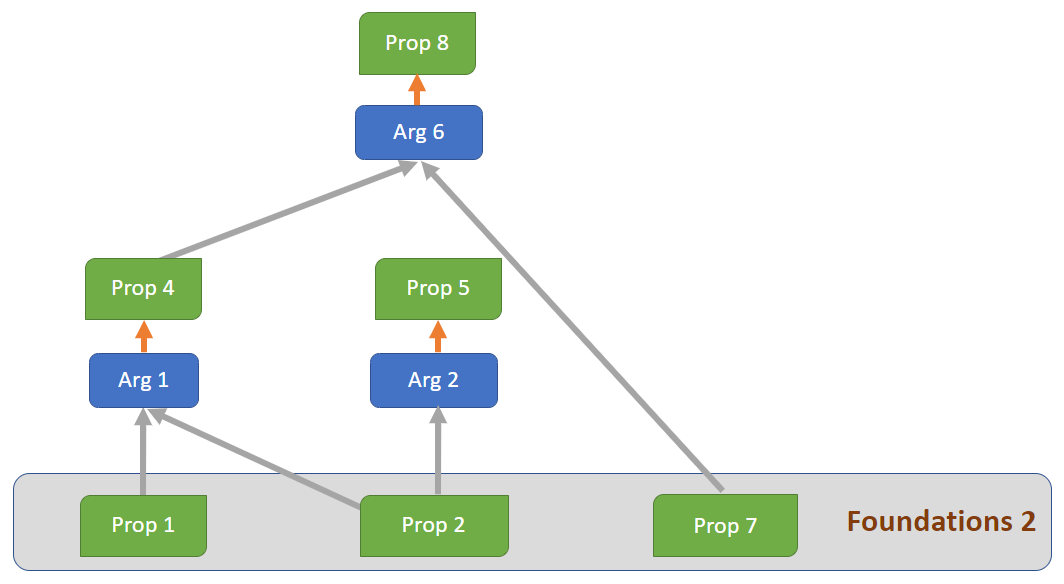
\includegraphics[height=5cm]{proof_graph2}}
\caption{Proof graph from the same argument graph (Fig.~\ref{argument_graph}) using `Prop 1', `Prop 2', and Prop 7' as axioms.}
\label{proof_graph2}
\end{center}
\end{figure}

\subsection{Validity of Arguments}

The correctness of proofs obtained by the above process is contingent on the validity of the arguments in the argument graph. The validity of an argument is, in principle, independent of other arguments and objectively verifiable. Formally defined logistic systems indeed have a mechanical procedure to independently verify the validity of arguments.

However, only a small section of Mathematics is developed using formally verified arguments. The vast majority of mathematics is verified via peer review, and some of this knowledge is curated by experts in books, encyclopaedias. The claim of validity of proofs (arguments) is judged based on various parameters such as the academic standing of the claimant, the reputation of the peer reviewing journal, the history of errors in the book or encyclopaedia containing them, etc. Clearly, these criteria are subjective and each individual's criteria for accepting the validity of an argument can vary to some extent.

Sophize doesn't promote or endorse any criteria. Instead, it allows its users to choose the criteria they believe in. The validity criterion is modelled as a proposition and is attached to arguments as a premise. 

\begin{figure}[!ht]
\begin{center}
\fbox{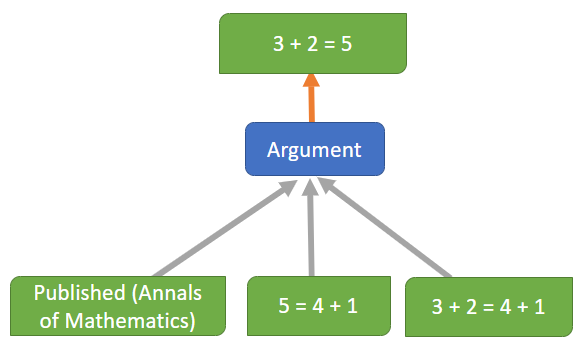
\includegraphics[height=3cm]{validity_criterion}}
\caption{Validity criteria as an argument premise.}
\label{validity_criterion}
\end{center}
\end{figure}

To easily manage validity criteria, the relationships between validity criteria are also maintained in the argument graph using arguments such as "Published in journal with SJR score $>$ 0.67" $\rightarrow$ "Published in Annals of Mathematics" (validation criterion should be provided for such arguments too). By maintaining such relationships, Sophize allows its users to conveniently choose multiple sources they consider to be reliable with a single manually chosen criterion. 

\subsection{Belief Sets}
\label{sec:bset}

A proposition is true if it is the conclusion of a valid argument and the premises of the argument are also true. Of course, this means that we need to start with some propositions that are assumed to be true without further justification. Traditionally, these are mathematical axioms and are considered to be self-evidently true. In mathematical inquiry, theorems are proven/disproven in one or more theories, each with its own set of axioms. Each theory may have its theoretical advantages and practical uses and there is no universal basis to choose one theory over another when trying to assert a proposition's truth/falsity.

Sophize allows any set of propositions to be considered true without evidence. Such a set of propositions is called a \textbf{belief set}. Propositions representing argument validity criteria are also part of belief sets. All propositions that are considered to be true in a belief set without proof are called its `unsupported propositions'. In addition, a belief set can also contain a number of `proof-generating machines' (e.g. for managing axiom-schemas) that will be discussed later. For ease of use, belief sets can also contain other belief sets.

The truth-value of a proposition is only defined within a belief set - there is no notion of absolute or universal truth on the Sophize platform. Sophize maintains proof graphs for all its belief sets.

\subsection{Tracking Inconsistencies}
If a proposition and its negation is proved within a belief set, it is inconsistent. As noted by the principle of explosion, any proposition can be proved from such a contradiction, thus making the claim of truth of any proposition practically worthless.

Thus, it is important to track and report contradictions in a belief set. To do that Sophize has a semantic notion of negation of a proposition. The premises or conclusion of an argument can be negations of propositions. When a proposition and its negation are proven, the system reports such contradictions for every belief set. When generating proof graphs from the argument graph, a contradicting proposition cannot be used a premise for any argument.

\subsection{Potential Advantages}

Logical organization of mathematics can lead to many advantages. We list some interesting ones below.

This knowledge organization scheme facilitates the re-use of propositions, and arguments across different theories. For example, to organize knowledge of different constant-curve geometries, we would create 4 belief sets - one each for absolute, Euclidean, hyperbolic and elliptic geometries. The latter three belief sets would comprise the absolute geometry belief set and the appropriate version of the parallel postulate needed for them. In such a scheme all the arguments (proofs) added to the argument graph for absolute geometry would automatically be shared by the other three geometries. The other three geometries need to only add the arguments that utilize their version of the parallel postulate.

Another use case would be to understand the consequences of important conjectures like the Reimann hypothesis by creating two belief sets - one where the conjecture is true and one where it is false. The proof graphs would systematically store such conjectural knowledge which often gets lost especially when results from multiple conjectures are involved. Complexity theory is one such field where this need is quite apparent. On a more practical note, several information security systems build on the conjectural developed with the assumption $P \neq NP$.

Proof graphs are currently organized as trees as seen in Fig \ref{proof_tree}. Users can keep exploring the proof till they reach a point where the propositions are already familiar to them. A future application of proof graphs would be to generate narrative proofs based on tailored to the reader's current understanding. This could be achieved in a classroom setting where the current level of mathematical understanding of students is known or assumed. It may also be possible to infer this from the user's activity on the platform.

\subsection{Limitations}
The scheme described in this section has a semantic notion of negation of a proposition to track contradictions. Thus it is incapable of organizing knowledge that depends on more complex calculi such as many-valued logics.

\section{Proof-Generating Machines (PGM)}
\label{sec:pgm}
A lot of mathematical knowledge is computed. Computation machines (e.g. calculators, algebras) can be seen as performing the following tasks
\begin{itemize}
\item Parsing the input into a language that can represent math formulae. 
\item Finding and outputting an equivalent form of the formula.
\end{itemize}
Thus, their focus is not on finding the proof but only finding the equivalent (simplified) representation of the input formula (Although many computer algebras do show the steps of the computation.). With Sophize, the focus instead is to generate proofs of the input propositions. A \textbf{proof-generating machine} (PGM) is a computer program that generates a partial proof graph against or in favour of an argument. PGMs can also have the capability to perform tasks 1 and 2, mentioned above.

PGMs take in some text as input which is parsed by the each PGM as they wish. Typically the text is treated either as a proposition (e.g. `3 + 5 = 8') or a formula (eg. `5+6') and in the latter case the PGM is responsible for finding an appropriate proposition (eg. `5 + 6 = 11') for the given input. The PGM then generates a proof graph for this proposition and returns back to the user.

The Sophize platform itself merely forwards the request to the associated PGM and performs some checks on the output returned. Any http server that can process a proof request can be easily plugged in to Sophize platform using its HTTP address. One server can implement multiple PGMs. An overview of PGMs generating Metamath proofs is here: \url{https://youtu.be/hJtEIo3ioLM}

\subsection{`Active' PGMs}
As with other parts of Sophize, the validity of the output of a PGM is not taken for granted. Each PGM must specify all the propositions (premises) that it will use in the root nodes of the proof graph it returns. In addition, a PGM may also delegate parts of proofs to another PGM. These PGMs must also be specified. Similar to argument validation criterion, each PGM should also have premise indicating PGM's correctness criteria (e.g. tested by X, verified by some committee, another program etc.)

A PGM is considered `active' in a belief set iff:
\begin{enumerate}
\item all of its premises are true in the belief set.
\item all the PGMs it delegates-to are active in the belief set.
\end{enumerate}

The output of a PGM is not used in belief sets in which it is not active.

\subsection{PGM Response}
The response of a request to any PGM has the following components:

\begin{itemize}

\item Truth value, i.e., whether the PGM considers the input proposition (provided or computed) true or false. PGM can also indicate that it doesn't understand the input or can't prove/disprove the proposition.

\item Proof graph (or a subset of proof graph) generated by the PGM in favour or against the input proposition. This component is skipped if only computation results are requested.
\end{itemize}

Note that unlike other propositions and arguments on Sophize, these are not stored on disk. They have a temporary URI specified in a slightly different format. The leaves of the DAG can have two kinds of arguments:

\begin{enumerate}
\item Arguments whose the premises are limited to the premises of the PGM.
\item Special `Arguments' that indicate that the generation of the proof of this argument's conclusion must be delegated to another PGM. To paginate large proofs, a PGM may also delegate to itself after generating some (say 100) arguments.
\end{enumerate}
\subsection{Materializing results}

Sophize allows saving the fact that a machine has returned a valid proof for a proposition (not the actual proof itself which can be quite large). Then this proposition can be used in further proofs without the need to invoke the proof generation every time. The proof, of course, can be requested by the users whenever required.


\section{Sophize Markdown}

In the author's view, it is crucial to maintain the proofs graphs for building trustable knowledge. However, the presentation of proofs as graphs to users is perhaps not very convenient. Traditional text-based narration remains indispensable when presenting knowledge to the reader.

We have extended the Markdown language - a lightweight markup language for creating formatted text using a plain-text editor - for building a rich narration interface. It allows users to quickly encode and present semantic data, to show the truth status of propositions available in prose, and to effortlessly access proof graphs. 

With Sophize Markdown, we can easily add \LaTeX\space by enclosing it between two \$ signs (or \$\$ for display math). A detailed specification of Sophize Markdown is available \cite{EasyChair6207} and many of its features are demonstrated at \url{https://youtu.be/5UYOpQwcjCk}. We highlight relevant features here:

\subsection{Embedding Semantic Data}

With Sophize Markdown we can easily link resources such as terms, propositions, and arguments. Links can be added using the pound sign (\#) and the resource's URI. There are multiple resource link options that can be used for changing the behaviour and text of the resource link. The following example utilizes some of the options.

\subsubsection*{Sample Markdown Code}

\begin{verbatim}
# Conic section

A conic section is a curve obtained as the intersection of the 
#(wiki/T_conical_surface, 'surface') of a #wiki/T_cone with a 
#wiki/T_plane. There are three types of conic sections.

## Ellipse
#oxford/T_ellipse|EXPAND #wiki/P_ellipse_area|EXPAND

## Parabola
...
\end{verbatim}

\paragraph{The above code is rendered as:}
\begin{mdframed}
\section*{Conic Section}
A conic section is a curve obtained as the intersection of the surface of a \dashuline{cone} with a \dashuline{plane}. There are three types of conic sections.

\subsection*{Ellipse}
An ellipse is a regular \dashuline{oval} shape, traced by a point moving in a plane so that the sum of its distances from two other points is constant. The area $A_{ellipse}$ enclosed by an ellipse is $$A_{ellipse} = \pi a b$$where $a$ and $b$ are the lengths of the \dashuline{semi-major} and \dashuline{semi-minor} axes, respectively.

\subsection*{Parabola}
...

\end{mdframed}

In the above example, the `EXPAND' option expanded the definition of the term, and statement of the proposition in place. Thus we were able to easily re-use concepts and theorems already extracted from other sources (say, Wikipedia and the Oxford dictionary in this case). Clicking on the underlined concepts, pops-up a modal dialog with the definition of the term clicked.

\subsection{Truth Status}

When a belief set is chosen, Sophize markdown adds an icon next to each proposition link. This icon indicates whether the proposition has been proven or dis-proven (or both) in the currently selected belief set using an appropriate symbol such as a check-mark or a cross. Clicking on the icon brings up the proof graph as shown in Fig.~\ref{proof_tree}. If the users switches from one belief set to another, the icon is updated based on the truth values in the new belief set but other parts of the article are unchanged. This functionality is demonstrated in the demo in subsection \ref{sec:sophize_proofs}. Similarly, an icon is added next to a proof generating machine which indicates whether the PGM is active or not.

\subsection{Formal Language Support}
In the case of formal languages, when propositions can be fully parsed, Sophize can automatically attach links to appropriate resources. This provides a convenient interface, where the user types in the native language, and the final output automatically allows users to explore all concepts that make up the input statement in depth. Currently, this is demonstrated in the use of Sophize Markdown with the Metamath language.

\section{Building a Modern Mathematics Library}
\label{sec:lib}
This sections discusses a some practical issues need to be overcome to build a modern scalable library with reliable information.

\subsection{Semantic Data Extraction}
Utilizing the full range of features offered by the Sophize platform requires the availability of semantic information. However, extracting semantic information from unstructured or semi-structured literature is a difficult problem. This problem can be seen as composed of several sub-problems:
\begin{itemize}
\item Finding definitions and propositions in prose.
\item Associating the appropriate entity with a term used in prose for quick lookup.
\item Identifying arguments along with premises and conclusion.
\item \label{prob:dup} Identifying duplicate definitions and propositions used in different sources.
\end{itemize}

Solving these problems would require manual effort (e.g. crowd-sourcing) combined with automated extraction tools. Recent progress in machine learning and natural language processing techniques \cite{ginev2019scientific} does make this problem seem tractable.

\subsection{Data Management}

Sophize divides its data into groups called datasets for copyright and data access management. For example, the 'wiki' dataset that extracts knowledge from Wikipedia mathematics glossaries releases its data under `CC-BY-SA' license, whereas the `metamath' dataset is public (`CC0'). Our signed-in users are free to create their own datasets and we allow them to choose who can read, write or comment in these datasets. Another interesting access control is the restriction of use of resources (especially argument-validity criteria) from an otherwise open-to-read dataset.

Information can be added to Sophize platform using intuitive web forms. However, it is infeasible to extract information from large repositories in this manner. Sophize publishes its data schema (explained in Section \ref{sec:core}) and helper libraries in multiple languages. The extracted information is can thus be stored as text (JSON) files in a repository. Sophize provides dataset owners the ability to sync knowledge such repositories to the central Sophize database.

\subsection{Search Interface}
\label{sec:search}
Sophize allows its users to run a run a federated search over its resources using an Elasticsearch server. We even allow users to \LaTeX to their search queries. The server runs search a space-insensitive and case-insensitive search over \LaTeX\space formulae by encoding \LaTeX\space formulae as lexemes and an Elasticsearch analyzer that removes spaces and lower cases the encoding. (See section \ref{sec:sources} for sources)

\subsection{Collaboration}

The Sophize platform includes an innovative mathematics communication interface designed to help our users discuss mathematics and collaboratively discover new proofs. The design focuses on making the collaboration more productive and enjoyable by building the right set of technical tools that aid in effective organization and summarization of existing progress. With Sophize Markdown at its core, Sophize's collaboration interface\cite{EasyChair6207}  (demo: \url{https://youtu.be/d3gaalJ7UQM}) is able to provide key features such as easy linking of existing math content, \LaTeX\space support, and live preview of comment drafts.


\section{Conclusion And Future Work}
\label{sec:conclusion}

We have presented the Sophize platform, a modern open mathematics library focused on providing reliable and detailed knowledge to its users. We extract and aggregate logical arguments from a wide variety of sources including published research, encyclopedias, formal theorem provers, and formal/informal programs. While there exist other systems that work with disparate data sources, we are aware of no other systems that attempt to logically aggregate knowledge across these data sources. Using this organization scheme we can maintain proofs of results from different theoretical foundations and tailor them to a user's knowledge reliability criterion.

We show how PGMs can be used to compute proofs in real-time and embed them in our knowledge graphs. We utilize the proof-graphs using Sophize Markdown to allow users to effortlessly browse proofs and lookup math entities in math literature. While there are other ways to represent semantic knowledge, such as content MathML and OpenMath, their scope is somewhat limited to specifying the meaning of the mathematical formula. The sTeX system \cite{Kohlhase2008} is perhaps most similar to Sophize Markdown but it needs creation of \LaTeX\space documents and use of \LaTeX ML systems. This makes its use in real-time web workflows impractical.

In its current state, Sophize has limited information to share with its users. Thus, we would first like to develop automated or semi-automated techniques to extract semantic knowledge from literature and expand the knowledge base that we share with our community. Using the proof-graphs and the semantic information collected we would like to make it easier for users to find relevant content with better search results.

\subsection*{Sources}
\label{sec:sources}
The source code for several aspects of the Sophize platform (include Sophize Markdown) is  at available at \url{https://github.com/Sophize}. The math encoder and Elasticsearch analyzer mentioned in section \ref{sec:search} are available at \url{https://gist.github.com/abc-sophize}.

\subsubsection{Acknowledgements} 
A part of the research presented here was supported by the International Mathematical Union.


\bibliographystyle{splncs04}
\bibliography{mybib}
\end{document}
